\chapter{Analyse de l'existant}

\section{Démarche d'analyse}

\noindent Pour évaluer le positionnement de \textbf{SecuCom} dans le paysage des solutions destinées aux secrétariats sociaux, une analyse des plateformes existantes a été menée selon plusieurs axes :

\begin{itemize}[leftmargin=*,label=\textcolor{darkgray}{$\bullet$},itemsep=0.3em]
  \item Étude documentaire des solutions leaders du marché belge
  \item Entretiens avec des utilisateurs actuels de ces plateformes
  \item Analyse comparative des fonctionnalités et modèles tarifaires
  \item Identification des forces et faiblesses par rapport aux besoins des petits secrétariats sociaux
\end{itemize}

\noindent Cette méthodologie a permis d'établir une cartographie de l'offre existante et d'identifier les opportunités pour \textbf{SecuCom}. Deux acteurs majeurs ont particulièrement retenu notre attention : EasyPay et Liantis.

\begin{note}
L'analyse s'est concentrée sur les fonctionnalités pertinentes pour les petits secrétariats sociaux, avec une attention particulière à la facilité d'utilisation, au coût et à l'adéquation avec les processus métier spécifiques.
\end{note}

\section{Analyse comparée des solutions}

\subsection{EasyPay}

\begin{figure}[H]
    \centering
    
\includegraphics[width=0.2\textwidth]{easyPayLogo.jpeg}
    \caption{Logo d'EasyPay Group \cite{easypay}}
    \label{fig:easyPayLogo}
\end{figure}

\newpage
\noindent \textbf{EasyPay} Group est un acteur incontournable dans le domaine des services de secrétariat social en Belgique, proposant une suite complète d'outils :

\begin{itemize}[leftmargin=*,label=\textcolor{darkgray}{$\bullet$},itemsep=0.3em]
  \item Gestion de la paie et des déclarations sociales
  \item Administration du personnel
  \item Gestion des temps et plannings
  \item Recrutement et développement des compétences
  \item Outils de reporting et digitalisation des processus RH
\end{itemize}

\noindent L'écosystème \textbf{EasyPay} se caractérise par sa richesse fonctionnelle et son approche intégrée, avec des modules interconnectés offrant une expérience cohérente.

\begin{figure}[H]
    \centering
    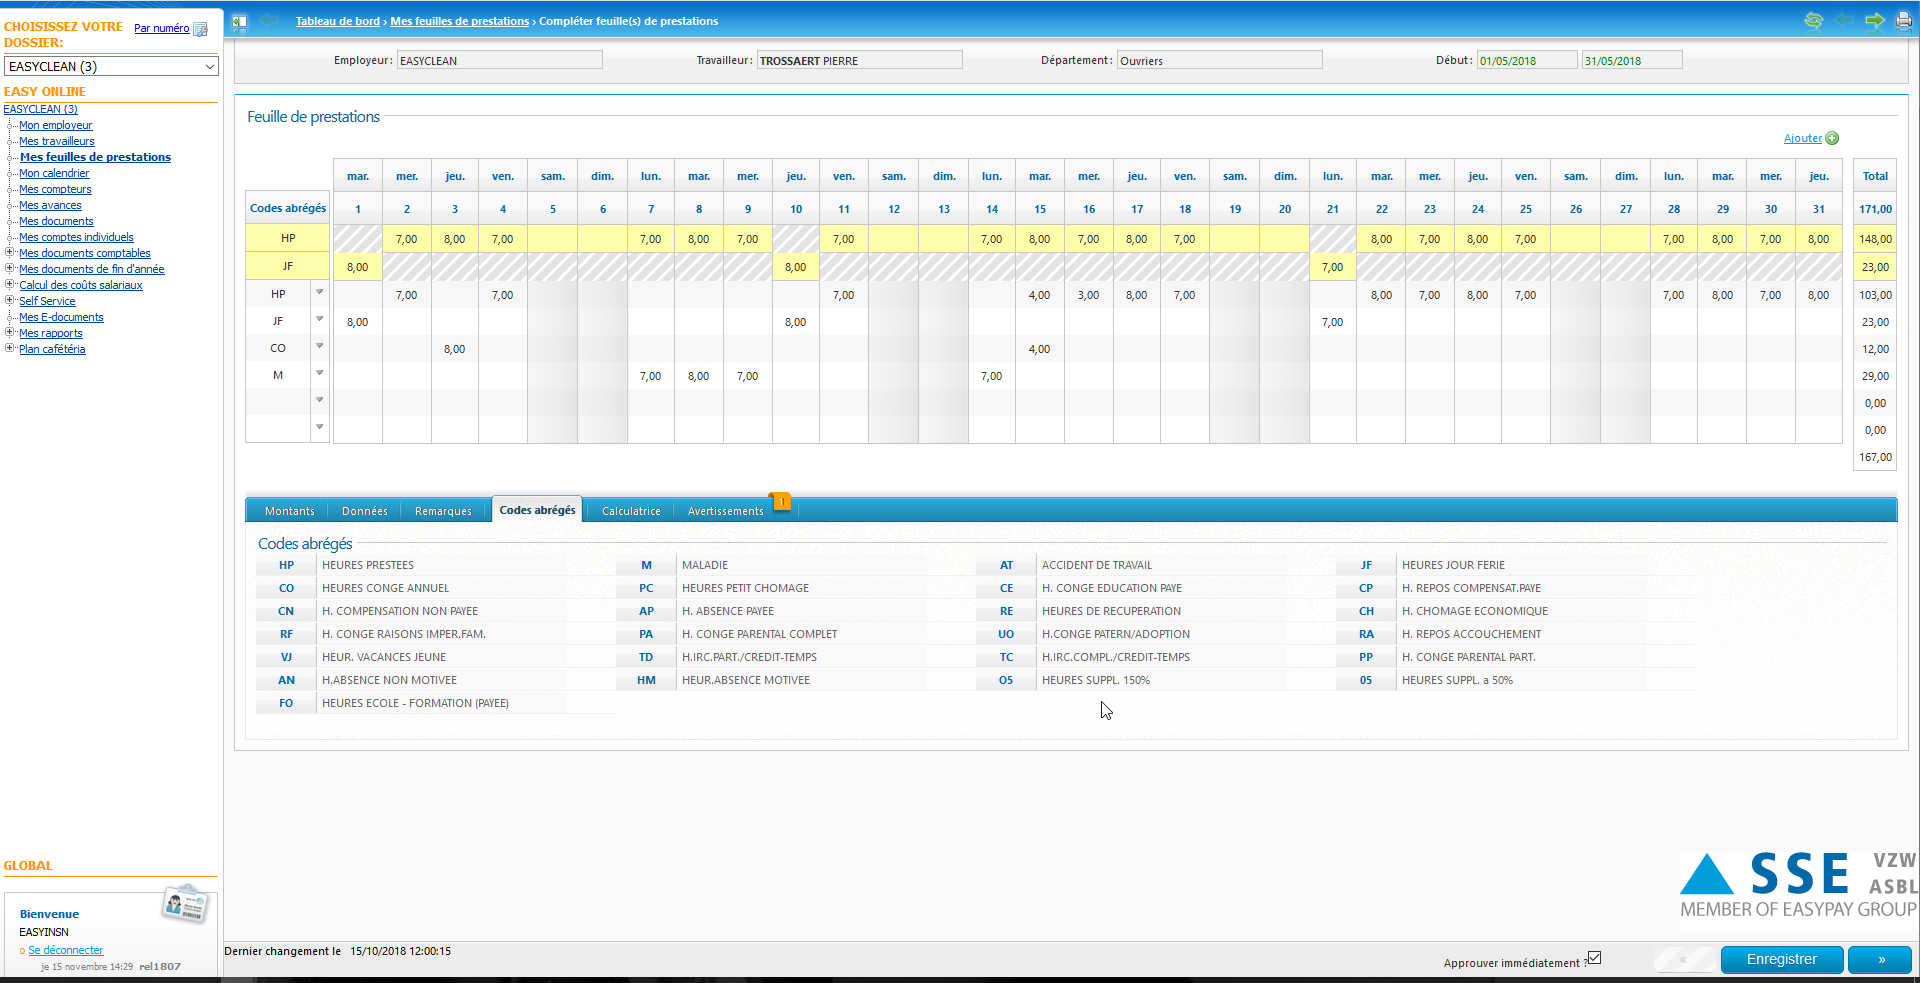
\includegraphics[width=0.9\textwidth]{easyPayScreenshot.png}
    \caption{Capture d'écran de l'interface d'EasyPay \cite{easypay}}
    \label{fig:easyPayScreenshot}
\end{figure}

\begin{tcolorbox}[
  title={\textbf{Limites pour les petites structures}},
  colback=blue!5!white,
  colframe=primarycolor,
  fonttitle=\bfseries,
  boxrule=0.5mm,
  arc=2mm,
  left=6mm,
  right=6mm,
  top=6mm,
  bottom=6mm
]
\noindent Cette exhaustivité constitue également le principal inconvénient d'\textbf{EasyPay} pour les petites structures comme Sodabel :
\begin{itemize}[leftmargin=*,label=\textcolor{darkgray}{$\bullet$},itemsep=0.3em]
  \item Complexité d'utilisation et de maîtrise
  \item Coût élevé de déploiement et maintenance
  \item Surdimensionnement par rapport aux besoins réels
  \item Rigidité des processus, limitant la personnalisation
\end{itemize}
\end{tcolorbox}

\newpage
\subsection{Liantis}

\begin{figure}[H]
    \centering
    
\includegraphics[width=0.2\textwidth]{liantisLogo.png}
    \caption{Logo de Liantis \cite{liantis}}
    \label{fig:liantisLogo}
\end{figure}

\noindent \textbf{Liantis} représente un autre acteur majeur du secteur, né de la fusion de plusieurs entités historiques du marché belge. Sa plateforme se distingue par son approche "guichet unique" :

\begin{itemize}[leftmargin=*,label=\textcolor{darkgray}{$\bullet$},itemsep=0.3em]
  \item Secrétariat social complet
  \item Assurances sociales pour indépendants
  \item Médecine du travail et prévention
  \item Allocations familiales et assurances diverses
  \item Conseil juridique et formation
\end{itemize}

\noindent La force de \textbf{Liantis} réside dans cette approche holistique permettant de gérer l'ensemble des obligations sociales via un seul partenaire.

\begin{figure}[H]
    \centering
    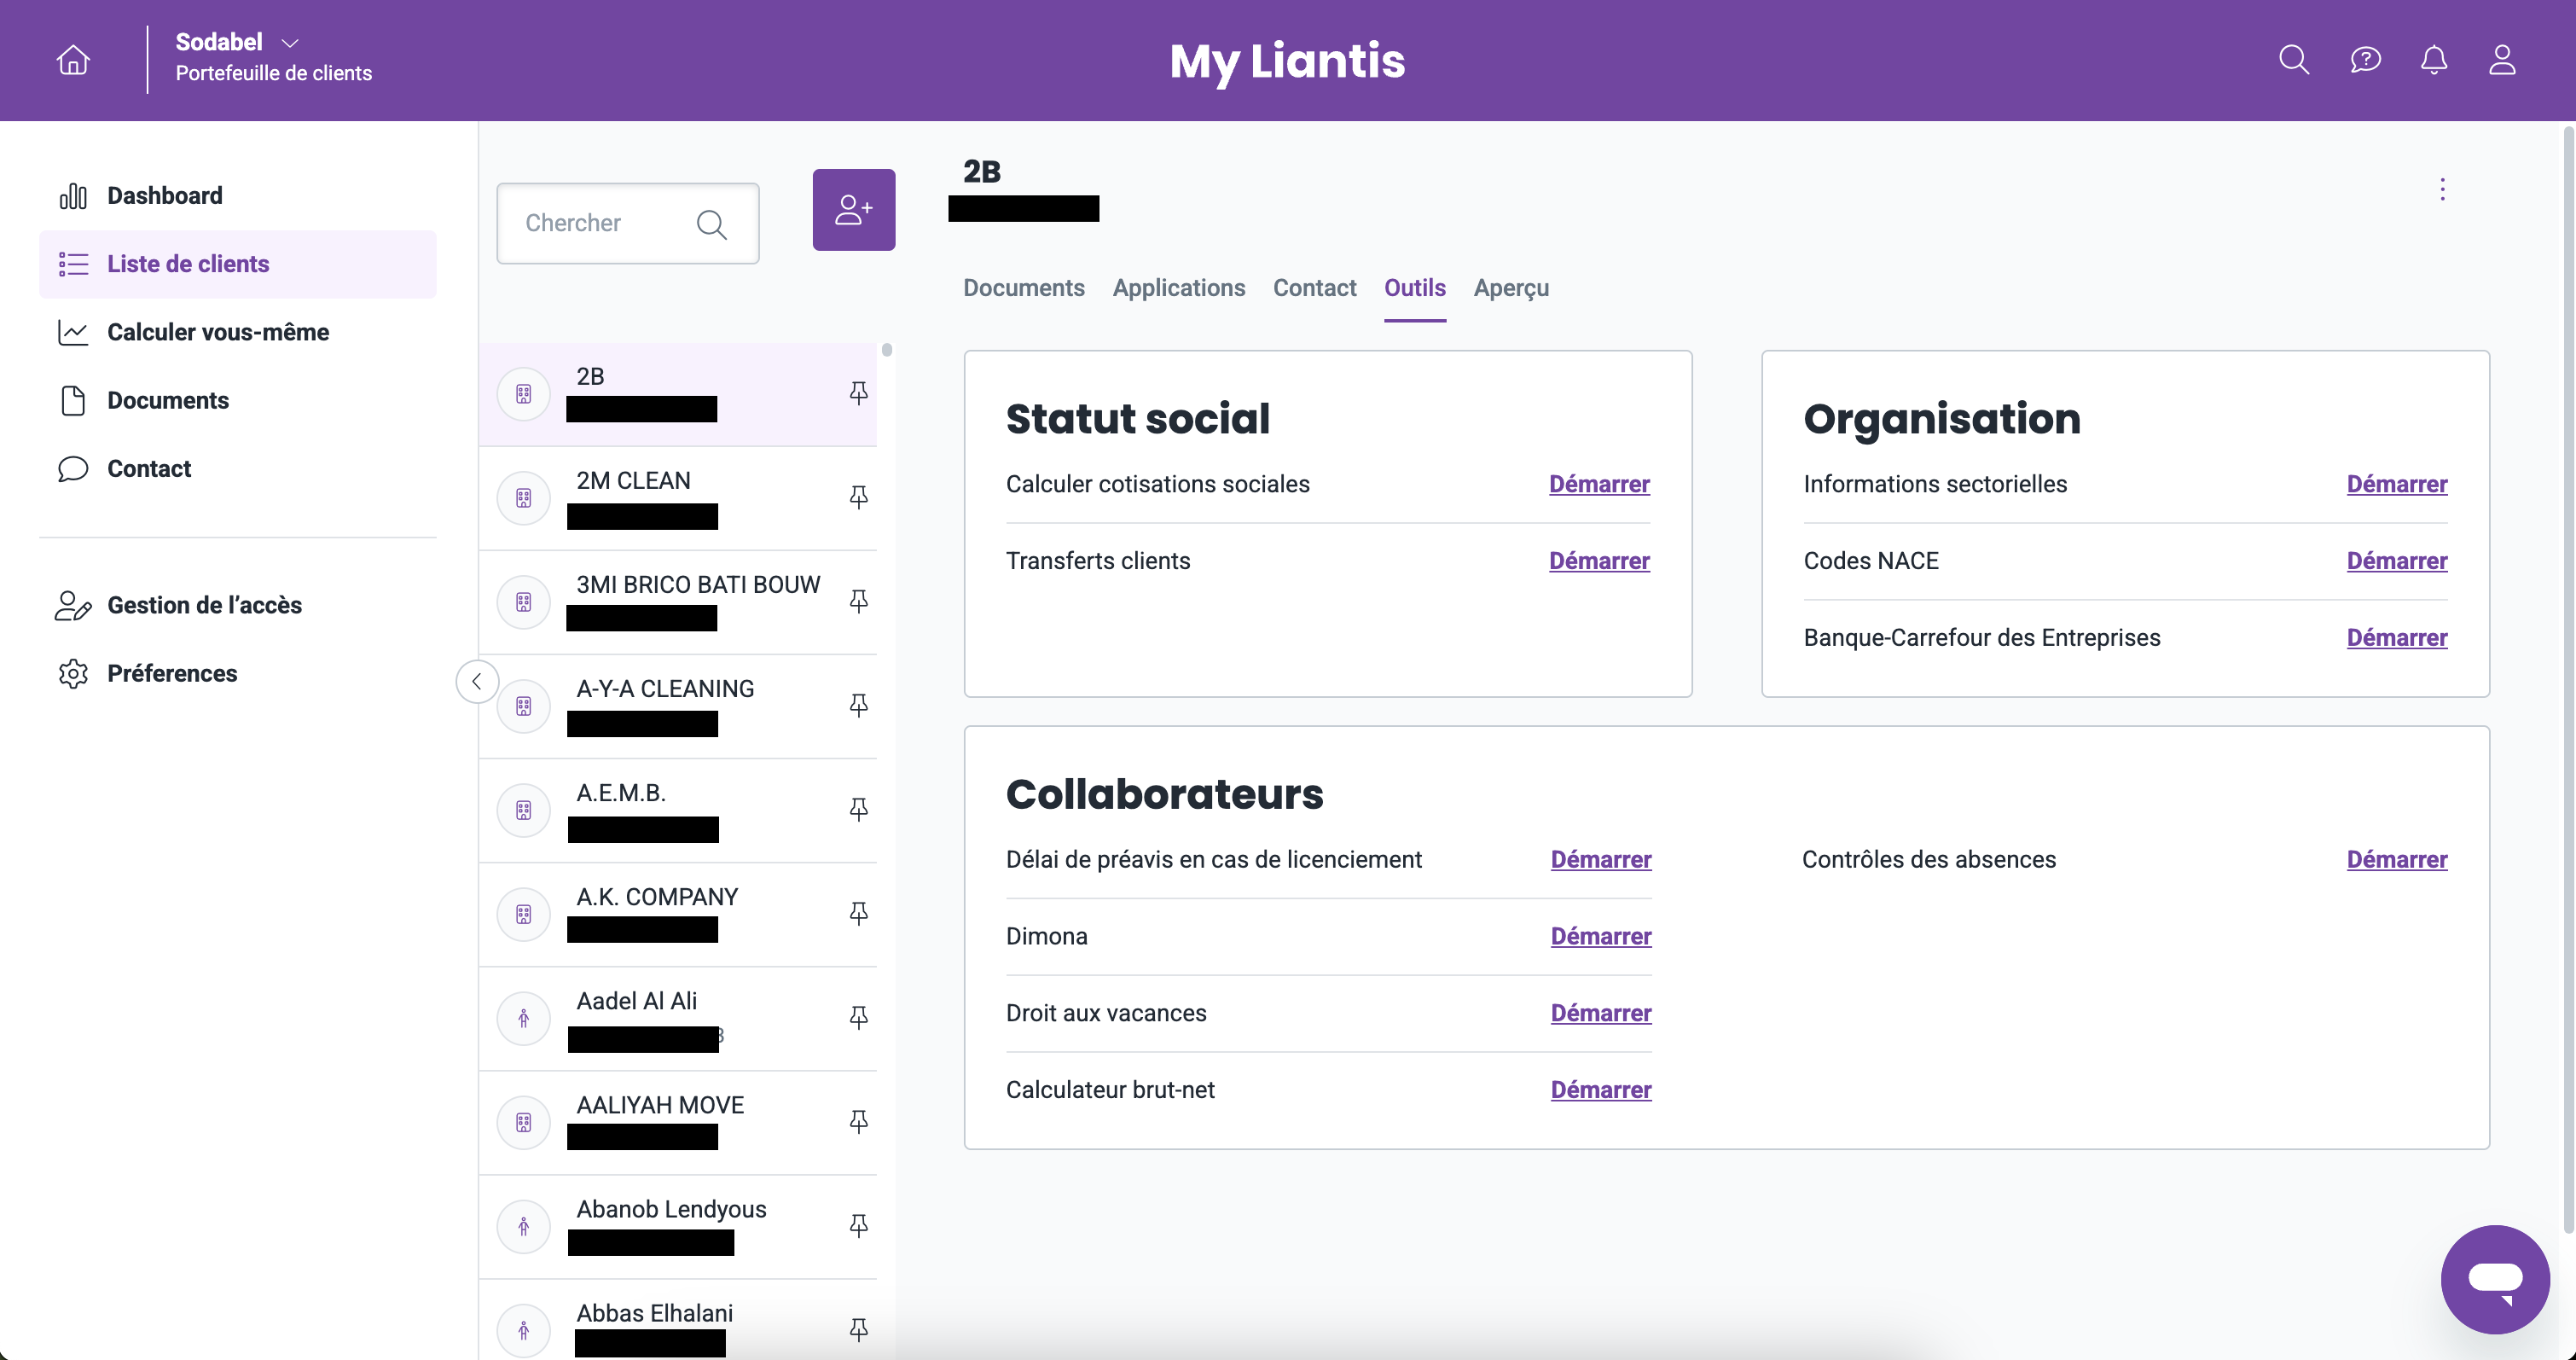
\includegraphics[width=0.9\textwidth]{liantisScreenshot.png}
    \caption{Capture d'écran de l'interface de Liantis \cite{liantis}}
    \label{fig:liantisScreenshot}
\end{figure}

\begin{tcolorbox}[
  title={\textbf{Contraintes pour les petites structures}},
  colback=blue!5!white,
  colframe=primarycolor,
  fonttitle=\bfseries,
  boxrule=0.5mm,
  arc=2mm,
  left=6mm,
  right=6mm,
  top=6mm,
  bottom=6mm
]
\noindent Cette exhaustivité s'accompagne de contraintes significatives :
\begin{itemize}[leftmargin=*,label=\textcolor{darkgray}{$\bullet$},itemsep=0.3em]
  \item Structure tarifaire complexe et onéreuse
  \item Lourdeur administrative inhérente
  \item Processus standardisés manquant de souplesse
  \item Interface utilisateur parfois confuse due à la multitude de fonctionnalités
\end{itemize}
\end{tcolorbox}

\newpage
\section{SecuCom face à l'existant}

\noindent \textbf{SecuCom} se distingue d'\textbf{EasyPay} et \textbf{Liantis} par son approche ciblée et minimaliste. Là où ces plateformes couvrent l'intégralité du spectre des besoins administratifs, \textbf{SecuCom} se concentre exclusivement sur l'optimisation des processus de gestion des entreprises clientes, de leurs collaborateurs et des déclarations DIMONA.

\begin{tcolorbox}[
  title={\textbf{Avantages distinctifs de SecuCom}},
  colback=blue!5!white,
  colframe=primarycolor,
  fonttitle=\bfseries,
  boxrule=0.5mm,
  arc=2mm,
  left=6mm,
  right=6mm,
  top=6mm,
  bottom=6mm
]
\noindent Les avantages distinctifs de \textbf{SecuCom} sont multiples :

\begin{itemize}[leftmargin=*,label=\textcolor{darkgray}{$\bullet$},itemsep=0.3em]
  \item \textbf{Simplicité et intuitivité} : Interface épurée, focalisée sur l'essentiel
  \item \textbf{Coût optimisé} : Structure tarifaire adaptée aux petites structures
  \item \textbf{Flexibilité maximale} : Adaptation rapide aux processus spécifiques
  \item \textbf{Prise en main immédiate} : Courbe d'apprentissage réduite
  \item \textbf{Focus sur l'essentiel} : Optimisation des fonctionnalités quotidiennes
\end{itemize}
\end{tcolorbox}

\vspace{0.5cm}

\noindent Le tableau comparatif ci-dessous met en évidence le positionnement de \textbf{SecuCom} face à \textbf{EasyPay} et \textbf{Liantis} :

\begin{table}[H]
\caption{Comparaison des solutions pour secrétariats sociaux}
\label{tab:comparaison-solutions}

\makebox[\textwidth][c]{%
\renewcommand{\arraystretch}{1.3}
\begin{tabular}{p{3.2cm}p{4.2cm}p{4.2cm}p{4.2cm}}
\toprule
\rowcolor{darkgray} \textcolor{white}{\textbf{Critère}} & \textcolor{white}{\textbf{SecuCom}} & \textcolor{white}{\textbf{EasyPay}} & \textcolor{white}{\textbf{Liantis}} \\
\midrule

\textbf{Étendue fonc\-tionnelle} & 
\textbf{Ciblée} \newline
\small{Gestion entreprises, collaborateurs,\ DIMONA} & 
\textbf{Complète} \newline
\small{Paie, RH, temps, recrutement, etc.} & 
\textbf{Très large} \newline
\small{Social, assurances, médecine du travail, etc.} \\
\midrule

\textbf{Complexité d'utilisation} & 
\textcolor{green!70!black}{\small\textbf{Faible}} \newline
\small{Interface minimaliste} & 
\textcolor{orange!70!black}{\small\textbf{Élevée}} \newline
\small{Nombreux modules interconnectés} & 
\textcolor{red!70!black}{\small\textbf{Très élevée}} \newline
\small{Écosystème complet} \\
\midrule

\textbf{Coût relatif} & 
\textcolor{green!70!black}{\small\textbf{Optimisé}} \newline
\small{Adapté aux petites structures} & 
\textcolor{orange!70!black}{\small\textbf{Élevé}} \newline
\small{Licence + modules} & 
\textcolor{red!70!black}{\small\textbf{Très élevé}} \newline
\small{Services multiples} \\
\midrule

\textbf{Personnalisation} & 
\textcolor{green!70!black}{\small\textbf{Élevée}} \newline
\small{Adaptable aux processus spécifiques} & 
\textcolor{orange!70!black}{\small\textbf{Moyenne}} \newline
\small{Paramétrage dans cadre défini} & 
\textcolor{red!70!black}{\small\textbf{Faible}} \newline
\small{Processus standardisés} \\
\midrule

\textbf{Temps de prise en main} & 
\textcolor{green!70!black}{\small\textbf{Court}} \newline
\small{Quelques heures} & 
\textcolor{orange!70!black}{\small\textbf{Long}} \newline
\small{Plusieurs jours} & 
\textcolor{red!70!black}{\small\textbf{Très long}} \newline
\small{Plusieurs semaines} \\
\midrule

\textbf{Cible principale} & 
\textbf{Petits secrétariats sociaux} \newline
\small{Structures indépendantes} & 
\textbf{Moyennes et grandes entreprises} \newline
\small{Besoins diversifiés} & 
\textbf{Tout type d'entreprise} \newline
\small{Et d'indépendant} \\
\bottomrule
\end{tabular}%
}
\end{table}

\noindent En définitive, \textbf{SecuCom} ne cherche pas à remplacer des plateformes comme \textbf{EasyPay} ou \textbf{Liantis}, mais à offrir une alternative ciblée pour les secrétariats sociaux qui privilégient la simplicité et l'efficacité. Dans un marché dominé par des solutions complètes mais complexes, \textbf{SecuCom} répond au besoin de retour à l'essentiel avec des outils adaptés à des cas d'usage spécifiques.

\vspace{0.5cm}

\begin{tcolorbox}[
  title={\textbf{Évolutivité de SecuCom}},
  colback=blue!5!white,
  colframe=primarycolor,
  fonttitle=\bfseries,
  boxrule=0.5mm,
  arc=2mm,
  left=6mm,
  right=6mm,
  top=6mm,
  bottom=6mm
]
\noindent \textbf{SecuCom} est conçu comme une plateforme évolutive. Bien que la version actuelle se concentre sur les fonctionnalités essentielles, le projet prévoit des phases d'évolution futures pour enrichir progressivement l'application, tout en préservant sa philosophie de simplicité. Cette approche modulaire garantit que \textbf{SecuCom} pourra s'adapter aux besoins émergents sans tomber dans le piège de la surcharge fonctionnelle des solutions généralistes.
\end{tcolorbox}
